\documentclass[10pt]{beamer}
\usepackage{graphicx}
\usepackage{subfig}
\usepackage{color}
\usepackage{tikz}
	\usetikzlibrary{shapes.geometric, arrows}
	\usetikzlibrary{arrows,shapes,matrix}
	\usetikzlibrary{decorations.pathmorphing} 
	\usepgflibrary{plotmarks}
	\usetikzlibrary{patterns}  
	\usetikzlibrary{positioning} 
	\tikzstyle{roundedRectangle} = [rectangle, rounded corners, minimum width=3cm, minimum height=1cm,text centered, draw=black]
	\tikzstyle{link} = [thick, -]
	\tikzstyle{circleNode} = [circle, minimum size = 1cm, text centered, draw=black, inner sep=0.1cm]
	\tikzstyle{solidNode} = [circle,fill,inner sep=1pt]
	\tikzstyle{startstop} = [rectangle, rounded corners, minimum width=3cm, minimum height=1cm,text centered, draw=black]
	\tikzstyle{io} = [trapezium, trapezium left angle=70, trapezium right angle=110, minimum width=3cm, minimum height=1cm, text centered, draw=black]
	\tikzstyle{process} = [rectangle, minimum width=2cm, minimum height=1cm, text centered, draw=black, inner sep=0.1cm]
	\tikzstyle{decision} = [diamond, minimum width=2cm, minimum height=0cm, text centered, draw=black, inner sep=0cm]
	\tikzstyle{arrow} = [thick,->,>=stealth]
	\tikzstyle{branchnode} = [circle, minimum size = 1cm, text centered, draw=black, inner sep=0.1cm]
\usetheme{Copenhagen}

\title{Gurobi Workshop - Part II}
\author{Lan Peng, PhD Candidate}
\institute{Department of Industrial \& Systems Engineering\\University at Buffalo, SUNY}
\date{\today}

\begin{document}
	\begin{frame}[plain]
		\titlepage
	\end{frame}

	\begin{frame}
		\frametitle{Overview}
		\begin{itemize}
			\item Part I - 26th Oct.
			\begin{itemize}
				\item Introduction and Installation
				\item Manufactures Problem - Small Example of LP
				\item Parallel Machine Scheduling Problem - Simple Example of IP
				\item Traveling Salesman Problem - Lazy Constraints and Callback
			\end{itemize}
			\item Part II - 2nd Nov.
			\begin{itemize}
				\item Vehicle Routing Problem with Time Windows - Column Generation
				\item Facility Location Problem - Benders Decomposition
			\end{itemize}
		\end{itemize}
	\end{frame}

	\begin{frame}
		\vfill
		Special thanks to Dr. Walteros. I learned the material in this workshop from his lecture.
		\vfill
	\end{frame}

	\section{Column Generation and VRPTW}
	\begin{frame}
		\frametitle{VRPTW}
		Vehicle routing problem with time windows (VRPTW) can be defined as choosing routes for limited number of vehicles to serve a group of customers in the time windows. Each vehicle has a limited capacity. It starts from the depot and terminates at the depot. Each customer should be served exactly once. (From Hindawi)
		\begin{figure}[!h]
			\centering
			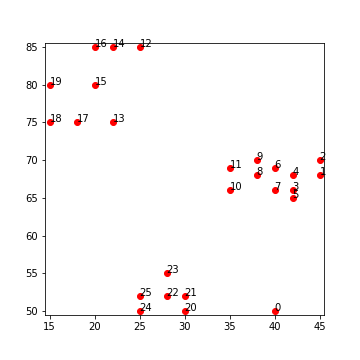
\includegraphics[width=0.5\textwidth]{VRPTW}
		\end{figure}
	\end{frame}

	\begin{frame}
		\frametitle{Set partitioning master problem}
		Create and select routes
		\begin{align*}
			\min \quad & \sum_{r \in Y} c_r y_r\\
			\text{s.t.} \quad & \sum_{r \in Y} y_r \le V\\
			& \sum_{r \in Y} a_{ir} y_r = 1, \quad \forall i \in C\\
			& y_r \ge 0 \quad (\text{Lower-bound searching}), \\
			\text{or}, \quad & y_r \in \{0, 1\} \quad (\text{Early branching})
		\end{align*}
		Set $Y$ is updated in each iteration.
	\end{frame}

	\begin{frame}
		\frametitle{Pricing subproblem}
		Finding the time-windowed shortest routes.
		\begin{align*}
			\min \quad & \sum_{(i, j) \in E} (c_{ij} - \pi_i) w_{ij}\\
			\text{s.t.} \quad & \sum_{j: (i, j) \in E} w_{ij} - \sum_{j:(j, i)\in E} w_{ji} = 0, \quad \forall i \in C \setminus \{0\}\\
			& \sum_{j: (0, j) \in E} w_{0j} = \sum_{j: (j, 0) \in E} w_{j0} = 1\\
			& \sum_{(i, j) \in E} w_{ij} d_{j} \le q \\
			& s_i + c_{ij} + t_i - M(1 - w_{ij}) \le s_j, \quad \forall i, j \in C\\
			& a_i \le s_i \le b_i, \quad \forall i \in C\\
			& w_{ij} \in \{0, 1\}, \quad \forall (i, j) \in E
		\end{align*}
	\end{frame}

	\begin{frame}
		\frametitle{Column Generation}
		\begin{figure}[!h]
			\centering
			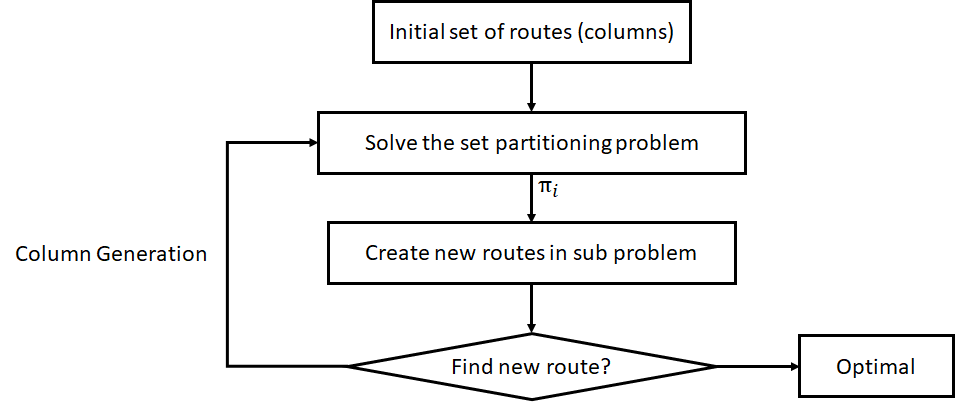
\includegraphics[width=1\textwidth]{CG}
		\end{figure}
	\end{frame}

	\section{Benders Decomposition and FLP}
	\begin{frame}
		\frametitle{Facility Location Problem}
		Consider the following facility location problem, where $m$ is the number of potential facilities, $n$ is the number of customers, and $\mathbb{Y}$ is the set of feasible plans of facility location plans, where $\mathbf{y} \subset \{0, 1\}^m \in \mathbb{Y}$. $c_{ij}$ is the cost for customer $i$ to be assigned to facility $j$, $d_j$ is the cost for opening facility $j$. The formulation is as following
		\begin{align*}
			\min \quad v& = \sum_{i = 1}^n \sum_{j = 1}^m c_{ij} x_{ij} + \sum_{j = 1}^m d_j y_j\\
			\text{s.t.} \quad & \sum_{j = 1}^m x_{ij} \ge 1, \quad \forall i \in \{1, 2, \ldots, n\}\\
				& x_{ij} \le y_j, \quad \forall i \in \{1, 2, \ldots, n\}, j \{1, 2, \ldots, m\}\\
				& x_{ij} \ge 0, \quad \forall i \in \{1, 2, \ldots, n\}, j \{1, 2, \ldots, m\}\\
				& y_{j} \in \{0, 1\}, \quad \forall j \in \{1, 2, \ldots, m\}
		\end{align*}
	\end{frame}

	\begin{frame}
		\frametitle{Sub problem}
		If $\mathbf{y}$ are \textbf{fixed}, i.e., $\mathbf{y} = \hat{\mathbf{y}} \in \mathbb{Y}$, the rest of the formulation will become a LP model with $x_{ij}$ as the nonnegative decision variables.
		\begin{align*}
			\min \quad v& = \sum_{i = 1}^n \sum_{j = 1}^m c_{ij} x_{ij} + \sum_{j = 1}^m d_j \hat{y}_j\\
			\text{s.t.} \quad & \sum_{j = 1}^m x_{ij} \ge 1, \quad \forall i \in \{1, 2, \ldots, n\}\\
				& x_{ij} \le \hat{y}_j, \quad \forall i \in \{1, 2, \ldots, n\}, j \{1, 2, \ldots, m\}\\
				& x_{ij} \ge 0, \quad \forall i \in \{1, 2, \ldots, n\}, j \{1, 2, \ldots, m\}\\
		\end{align*}
	\end{frame}

	\begin{frame}
		\frametitle{Dual of sub problem}
		 If we take the dual of the subproblem, we get
		\begin{alignat*}{2}
			\text{(Dual-Sub)} \quad v(\hat{\mathbf{y}}) = \max \quad & \sum_{i = 1}^n (\lambda_i - \sum_{j = 1}^m \hat{y}_j \pi_{ij}) + \sum_{j = 1}^m d_j \hat{y}_j \\
			\text{s.t.} \quad & \lambda_i - \pi_{ij} \le c_{ij} \quad \forall i \in \{1, 2, \ldots, n\}, j \in \{1, 2, \ldots, m\}\\
			& \lambda_i \ge 0 \quad \forall i \in \{1, 2, \ldots, n\}\\
			& \pi_{ij} \ge 0 \quad \forall i \in \{1, 2, \ldots, n\}, j \in \{1, 2, \ldots, m\}
		\end{alignat*}
	\end{frame}

	\begin{frame}
		\frametitle{Remind: Weak Duality theorem}
		\begin{table}
			\centering
			\begin{tabular}{c|c}
				Prime Problem & Dual Problem\\
				\hline
				Optimal & Optimal\\
				Unbounded or infeasible & Infeasible
			\end{tabular}
		\end{table}
	\end{frame}

	\begin{frame}
		\frametitle{Optimality Cuts and Feasibility Cuts}
		\begin{itemize}
			\item If the dual of sub problem has an optimal solution - add optimality cut
			\begin{equation*}
				\sum_{i = 1}^n \sum_{j = 1}^m c_{ij} x_{ij} \ge \sum_{i = 1}^n (\lambda_i - \sum_{j = 1}^m \pi_{ij} \hat{y}_j)
			\end{equation*}

			\item If the dual of sub problem is unbounded - add feasibility cut
			\begin{equation*}
				\sum_{i = 1}^n (\lambda_i - \sum_{j = 1}^m \pi_{ij} \hat{y}_j) \le 0
			\end{equation*}
			
			\item If the dual of sub problem is infeasible - terminate

		\end{itemize}
	\end{frame}

\end{document}